\documentclass[border=10pt]{standalone}
\usepackage{tikz}
\usetikzlibrary{automata, positioning, arrows.meta}

\begin{document}
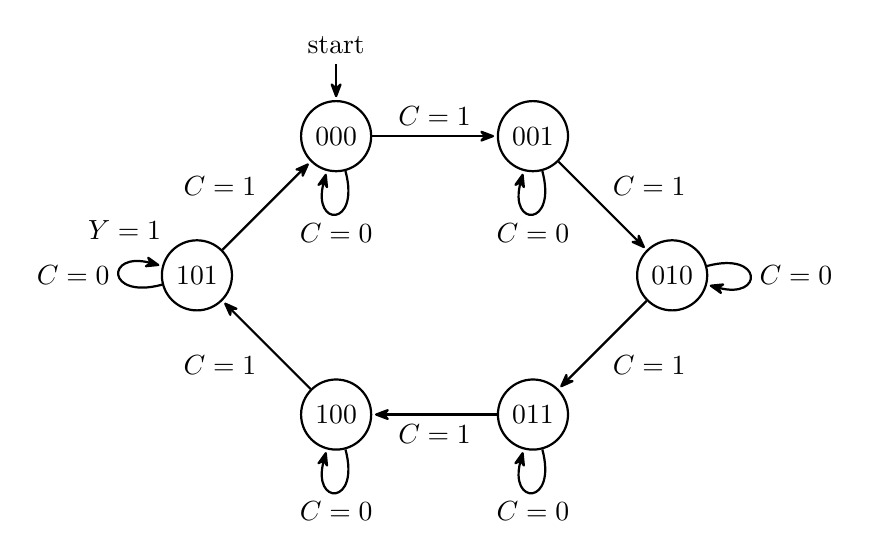
\begin{tikzpicture}[shorten >=1pt, node distance=2.5cm, on grid, auto, >={Stealth[round]}, thick]
    % Layout: Circular
    % States: 0 to 5
    
    \node[state, initial above] (s0) at (0, 0) {000};
    \node[state] (s1) [right=of s0] {001};
    \node[state] (s2) [below right=of s1] {010};
    \node[state] (s3) [below left=of s2] {011};
    \node[state] (s4) [left=of s3] {100};
    % State 5 has Output Y=1
    \node[state] (s5) [above left=of s4] {101};
    \node[above left] at (s5.north west) {$Y=1$};

    % Transitions
    % Loop s0->s1->s2->s3->s4->s5->s0 (C=1)
    % Self-loops (C=0)
    \path[->]
        (s0) edge node {$C=1$} (s1)
             edge [loop below] node {$C=0$} (s0)
        (s1) edge node {$C=1$} (s2)
             edge [loop below] node {$C=0$} (s1)
        (s2) edge node {$C=1$} (s3)
             edge [loop right] node {$C=0$} (s2)
        (s3) edge node {$C=1$} (s4)
             edge [loop below] node {$C=0$} (s3)
        (s4) edge node {$C=1$} (s5)
             edge [loop below] node {$C=0$} (s4)
        (s5) edge node {$C=1$} (s0)
             edge [loop left] node {$C=0$} (s5);

\end{tikzpicture}
\end{document}
